\documentclass[12pt, titlepage]{article}


% Author's up-front packages
\usepackage[T1]{fontenc}
\usepackage[utf8]{inputenc}
\usepackage{longtable}

%Packages from template
\usepackage{amsmath, mathtools}
%\usepackage[round]{natbib}
\usepackage{amsfonts}
\usepackage{amssymb}
\usepackage{graphicx}
\usepackage{colortbl}
\usepackage{xr-hyper}
\usepackage{hyperref}
\usepackage{xfrac}
\usepackage{tabularx}
\usepackage{float}
\usepackage{siunitx}
\usepackage{booktabs}
\usepackage{multirow}
\usepackage[section]{placeins}
\usepackage{caption}
\usepackage{fullpage}

% Author's packages

\usepackage{cite}
\usepackage{indentfirst}
\usepackage{csquotes}
\usepackage{cleveref}

\hypersetup{
%bookmarks=true,     % show bookmarks bar?
colorlinks=true,       % false: boxed links; true: colored links
linkcolor=red,          % color of internal links (change box color with linkbordercolor)
citecolor=blue,      % color of links to bibliography
filecolor=magenta,  % color of file links
urlcolor=cyan          % color of external links
}

\usepackage{array}

%% Comments

\usepackage{color}

\newif\ifcomments\commentstrue

\ifcomments
\newcommand{\authornote}[3]{\textcolor{#1}{[#3 ---#2]}}
\newcommand{\todo}[1]{\textcolor{red}{[TODO: #1]}}
\else
\newcommand{\authornote}[3]{}
\newcommand{\todo}[1]{}
\fi

\newcommand{\wss}[1]{\authornote{blue}{SS}{#1}}
\newcommand{\an}[1]{\authornote{magenta}{Author}{#1}}


\newcommand{\progname}{STEM Moir{\'e} GPA}
\externaldocument[SRS:]{../SRS/SRS}
\externaldocument[TP:]{../TestPlan/TestPlan}
\externaldocument[MG:]{../Design/MG/MG}
\externaldocument[MIS:]{../Design/MIS/MIS}
\externaldocument[T:]{../TestPlan/TestPlan}

%Set the custom referencing syste
	% Module
\newtheorem{M}{M}
\crefname{M}{M}{Ms}
	% Module Interface Specification
\newtheorem{MIS}{MIS}
\crefname{MIS}{MIS}{MISs}
	% Requirements
\newtheorem{R}{R}
\crefname{R}{R}{Rs}
	% Instance Model
\newtheorem{IM}{IM}
\crefname{IM}{IM}{IMs}
	% Test
\newtheorem{Test}{Test}
\crefname{Test}{Test}{Tests}

\begin{document}

\title{Test Report: STEM Moir{\'e} GPA} 
\author{Alexandre Pofelski \\
		macid: pofelska \\
		github: slimpotatoes}
\date{\today}
	
\maketitle

\pagenumbering{roman}

\section{Revision History}

\begin{tabularx}{\textwidth}{p{3cm}p{2cm}X}
\toprule {\bf Date} & {\bf Version} & {\bf Notes}\\
\midrule
18/12/2017 & 1.0 & First incomplete version to meet deadline\\
\bottomrule
\end{tabularx}

~\newpage

\section{Symbols, Abbreviations and Acronyms}

\renewcommand{\arraystretch}{1.2}
\begin{tabular}{l l} 
  \toprule		
  \textbf{symbol} & \textbf{description}\\
  \midrule 
  T & Test\\
  \bottomrule
\end{tabular}\\

\wss{symbols, abbreviations or acronyms -- you can reference the SRS tables if needed}

\newpage

\tableofcontents

\listoftables %if appropriate

\listoffigures %if appropriate

\newpage

\pagenumbering{arabic}

This document is providing information of \progname{} implementation by assessing the results of the tests designed in the TestPlan document. Regarding the size of \progname{} program, only a small part of the code has been tested in the required time frame therefore, only a few functional requirements have been evaluated. An important update to the document is planed once the implementation of the other tests are done.
\newline

For the moment, only a specific focus has been put on the \textbf{GPA Module} (\cref{MG:M_GPA} in the  MG document and \cref{MIS:MIS_GPA} in the MIS document) and the modules used by GPA which are:
\begin{itemize}
\item the \textbf{Data Structure Module} (\cref{MG:M_DataStruct} in MG document and \cref{MIS:MIS_DataStruct} in the MIS document)
\item the \textbf{Mask Module} (\cref{MG:M_Mask} in the MG document and \cref{MIS:MIS_Mask} in the MIS document)
\item the \textbf{Fourier Transform Module} (\cref{MG:M_FT} in MG document and \cref{MIS:MIS_FT} in the MIS document)
\item the \textbf{Gradient Module} (\cref{MG:M_Gradient} in MG document and \cref{MIS:MIS_Gradient} in the MIS document)
\item the \textbf{Phase Calculation Module} (\cref{MG:M_Phase} in MG document and \cref{MIS:MIS_Phase} in the MIS document)
\end{itemize}

\section{Functional Requirements Evaluation}

\textbf{Test \cref{SRS:R_7} in \cref{SRS:IM_2}}: Correctness of the GPA method application.\medskip

\textbf{\cref{T:T_Phase-Extraction-No-Strain}} from TestPlan document was designed to check if the gpa function of the GPA module outputs no strain with a simulated input signal with no strain. As a reminder, the GPA module is calculating $\Delta \overrightarrow{g}$ the variation of the wave vector $\overrightarrow{g}$ by isolating the spatial frequency $\overrightarrow{g}$ in Fourier space to extract the phase component. The variation of the phase is then related to the variation of the $\overrightarrow{g}$ wave vector using the gradient operation. \medskip

For {\cref{T:T_Phase-Extraction-No-Strain}} to run, a SMH has to be provided. The SMH has been generated using the numpy library by outputing a 2D array of (256,256) in size. Each element of the array represents the value of the sin function taken at the location of the array. The 2D array as a whole represents the sampled version of the 2D sin function and is a good representation of what is considered a STEM Moire hologram.  \Cref{fig:Test_2_explanation} is highlighting the results of{\cref{T:T_Phase-Extraction-No-Strain}} for the particular case described below:
\begin{itemize}
\item $I_{SMH_{exp}}=\sin{(2\pi g)}$, 
\item Mask $M$ of one pixel at $g\overrightarrow{u_x}$ in $\widetilde{I}_{SMH_{exp}}$
\end{itemize}

 

\begin{figure}[H]
\begin{center}
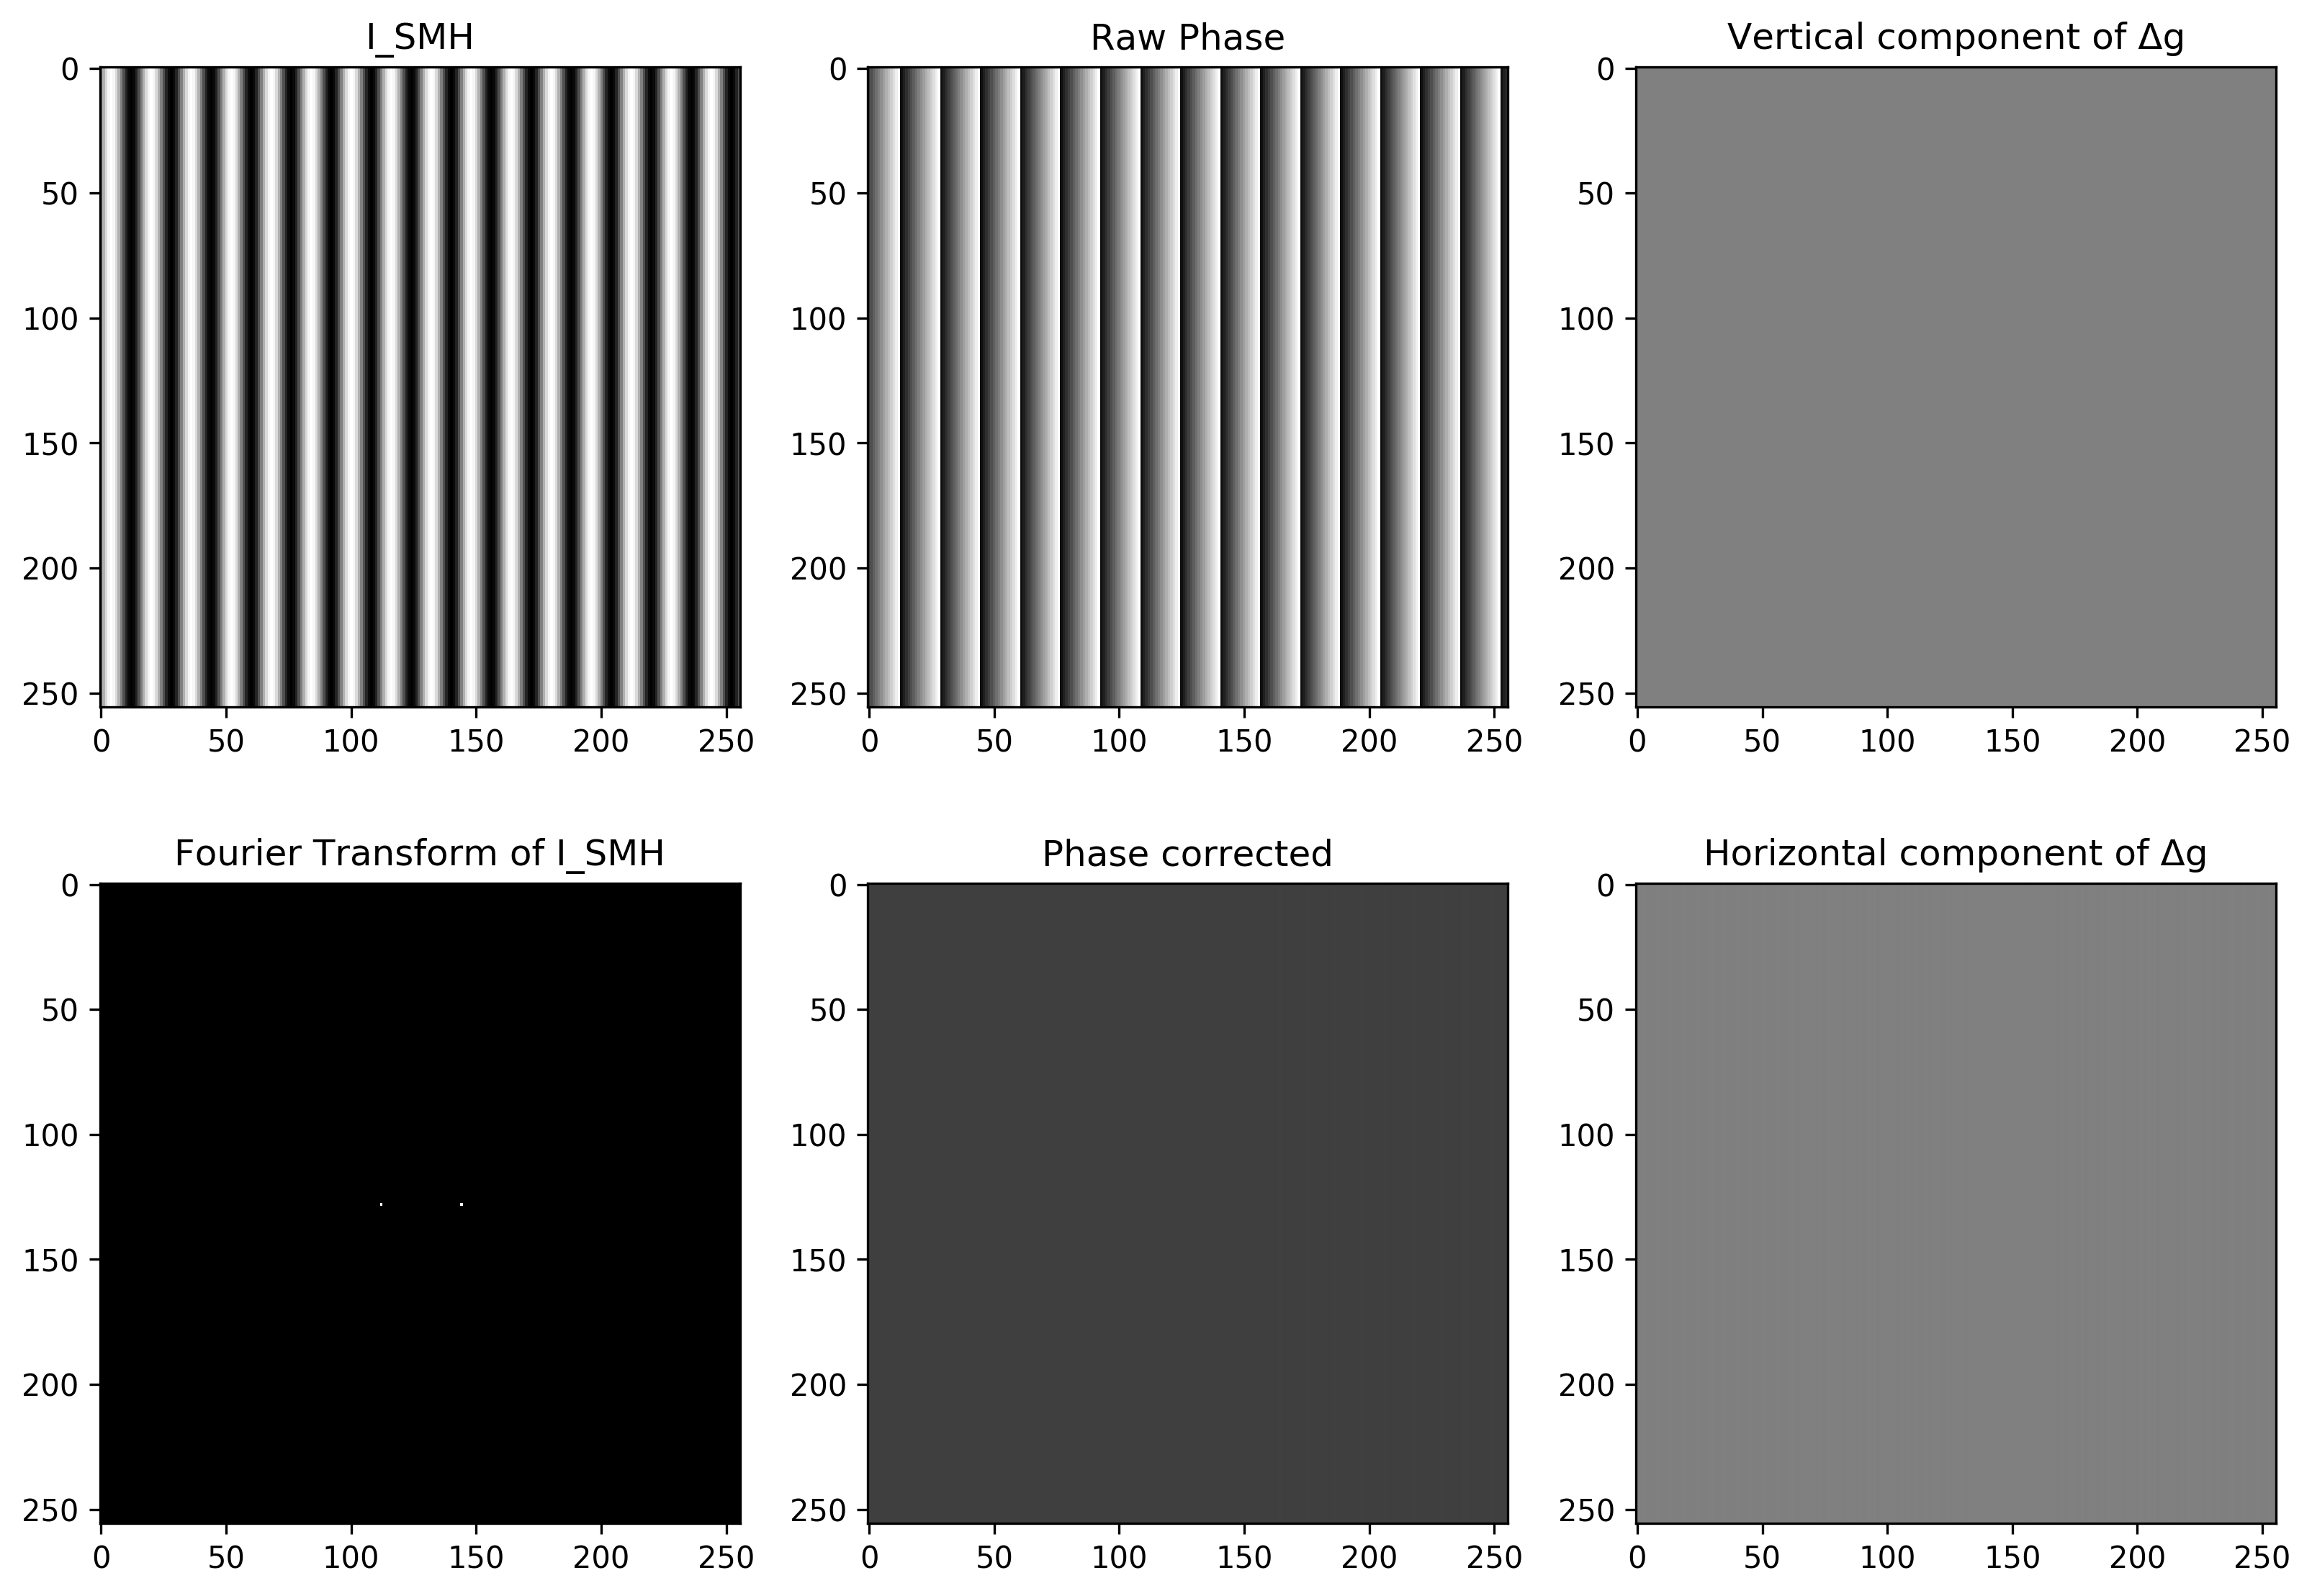
\includegraphics[scale=0.5]{Figures/Test_2_explanation.png}
\caption{}
\label{fig:Test_2_explanation}
\end{center}
\end{figure}

\begin{figure}[H]
\begin{center}
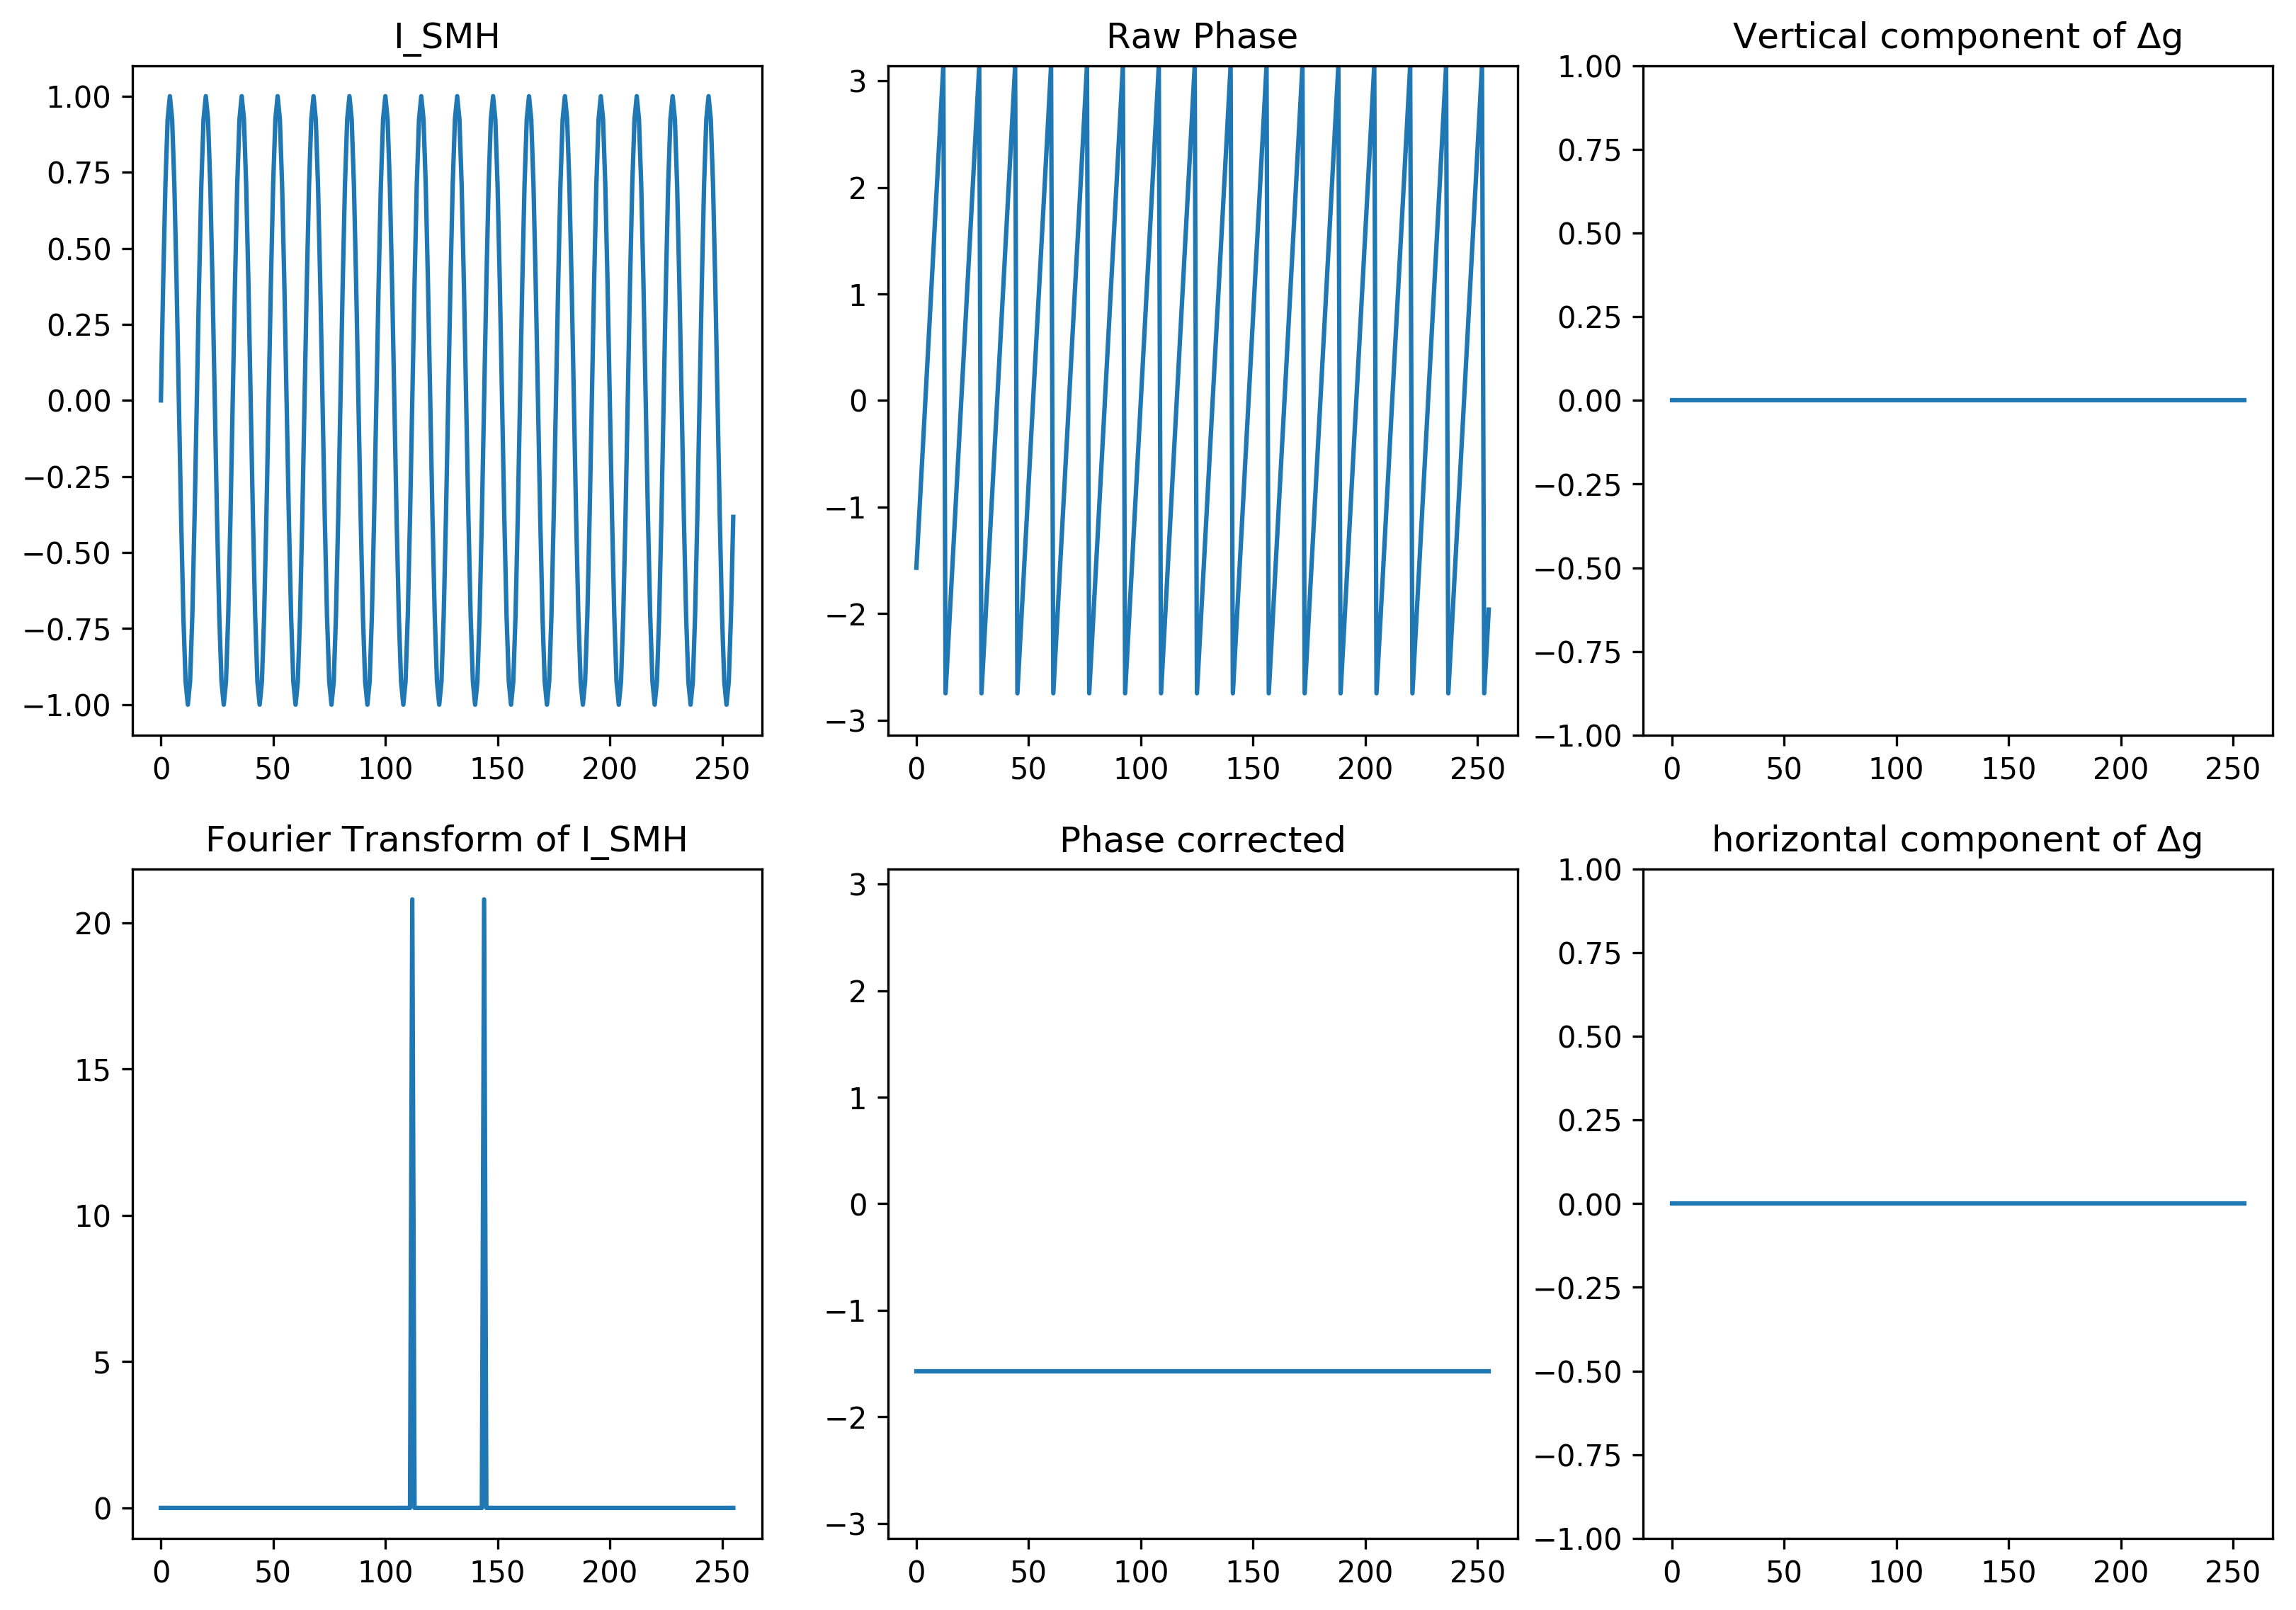
\includegraphics[scale=0.5]{Figures/Test_2_explanation_1D.png}
\caption{}
\label{fig:Test_2_explaination_1D}
\end{center}
\end{figure}

\begin{figure}[H]
\begin{center}
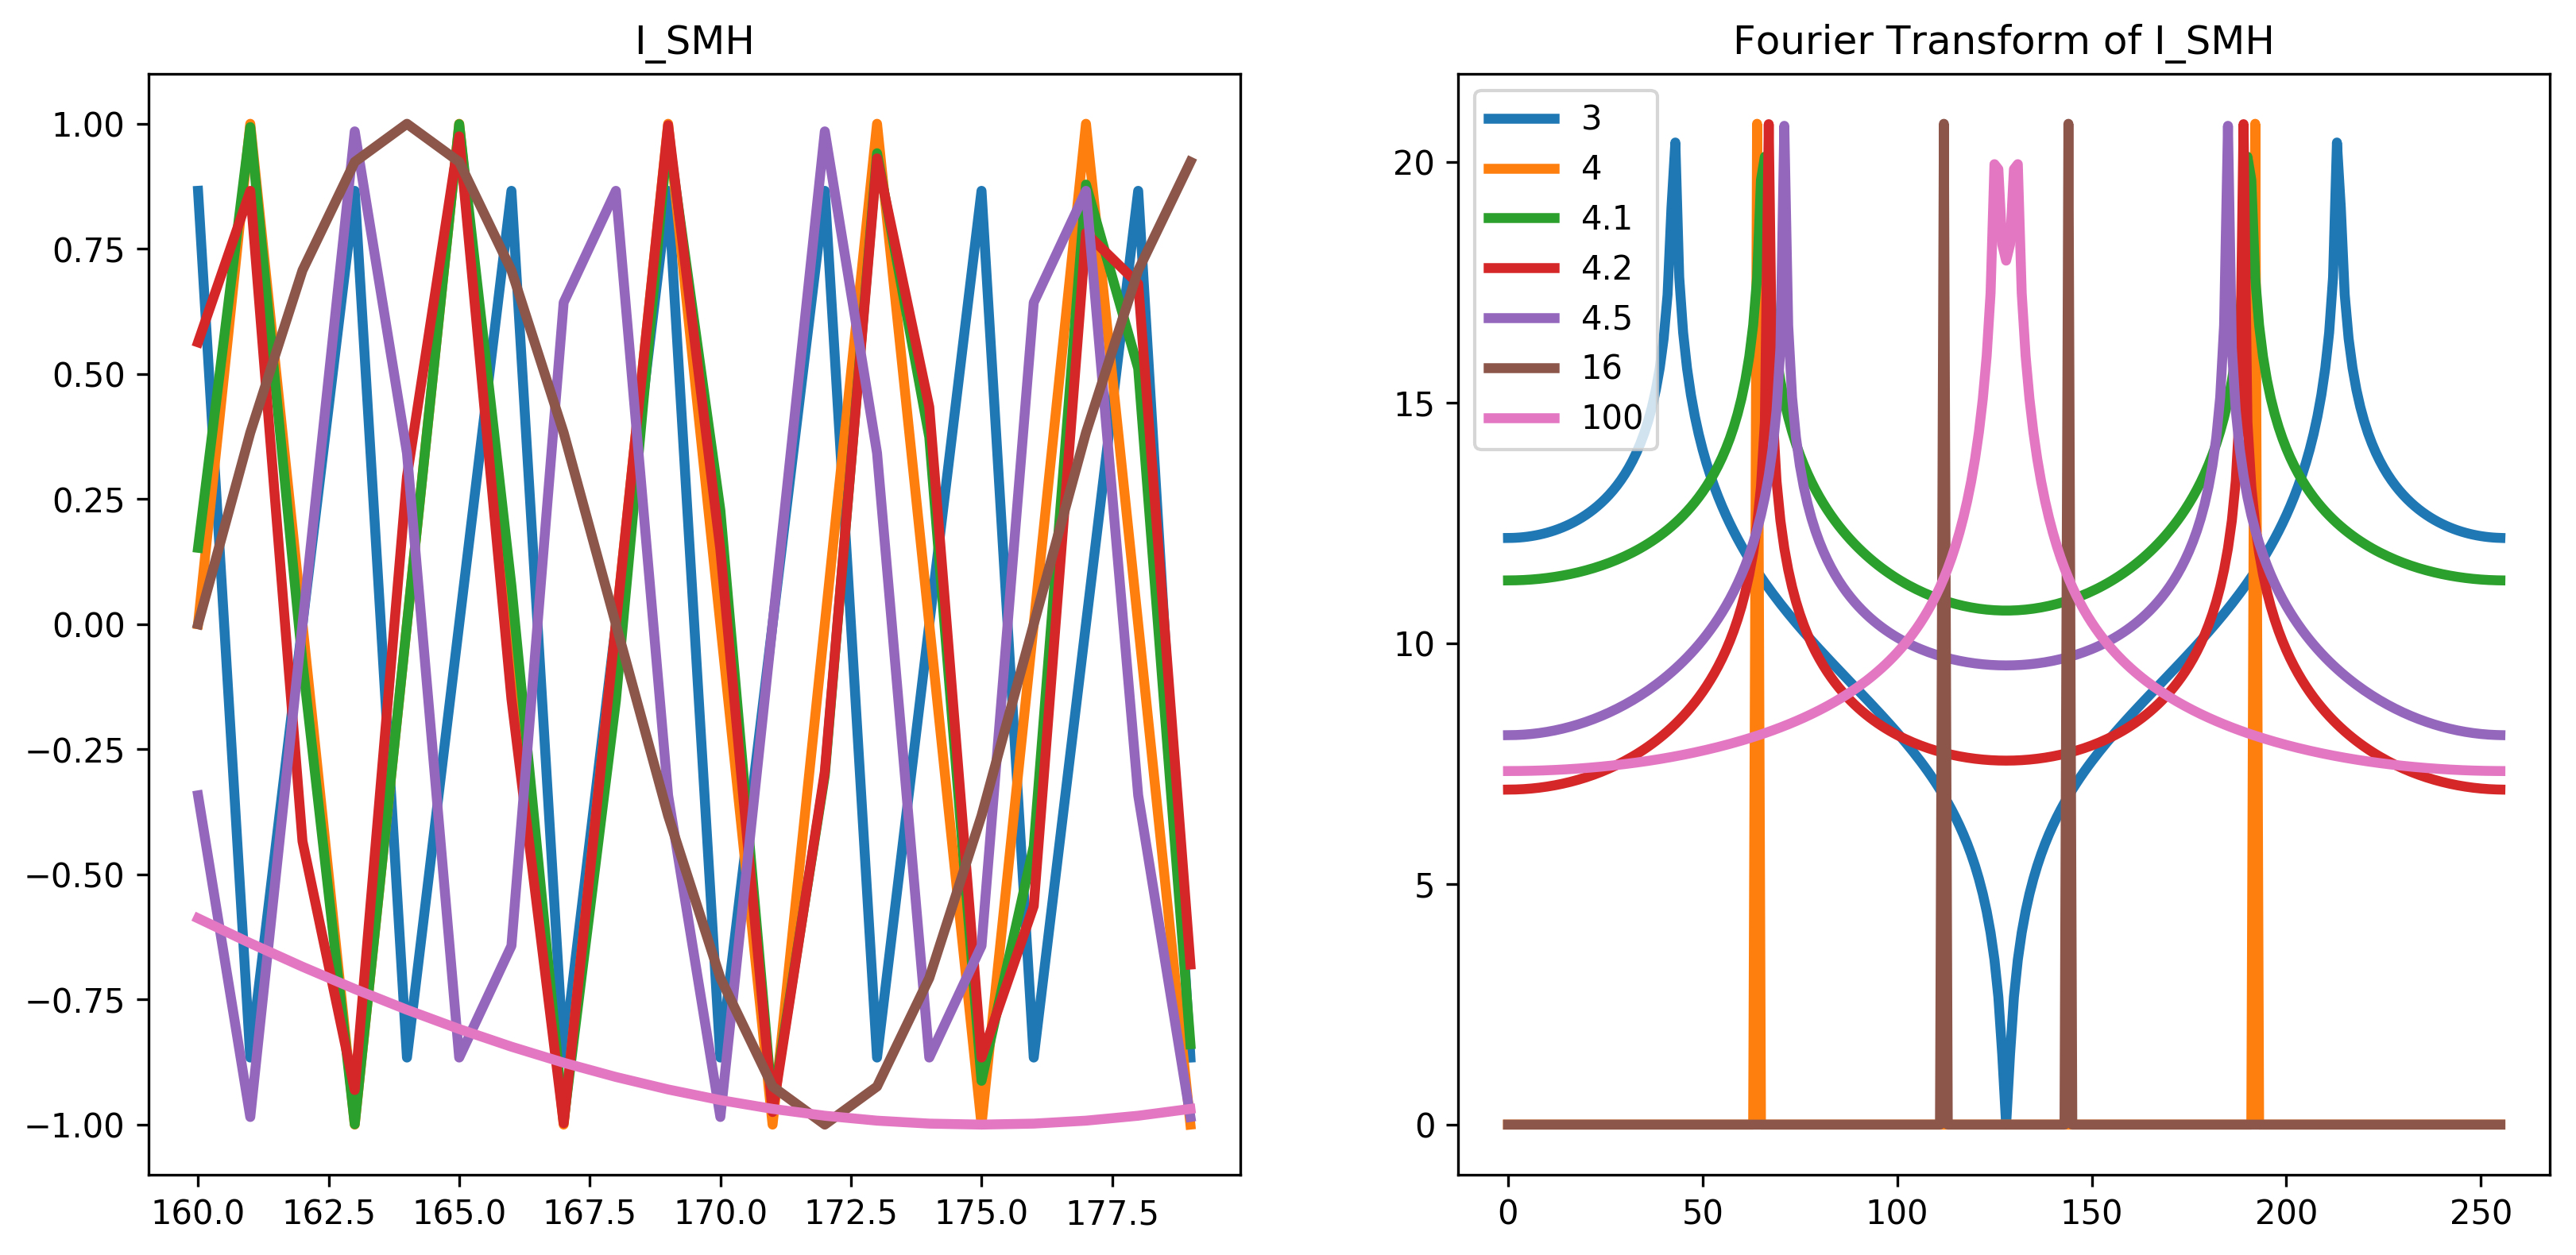
\includegraphics[scale=0.5]{Figures/Test_2_test_cases.png}
\caption{}
\label{fig:Test_2_Test_cases}
\end{center}
\end{figure}

\begin{figure}[H]
\begin{center}
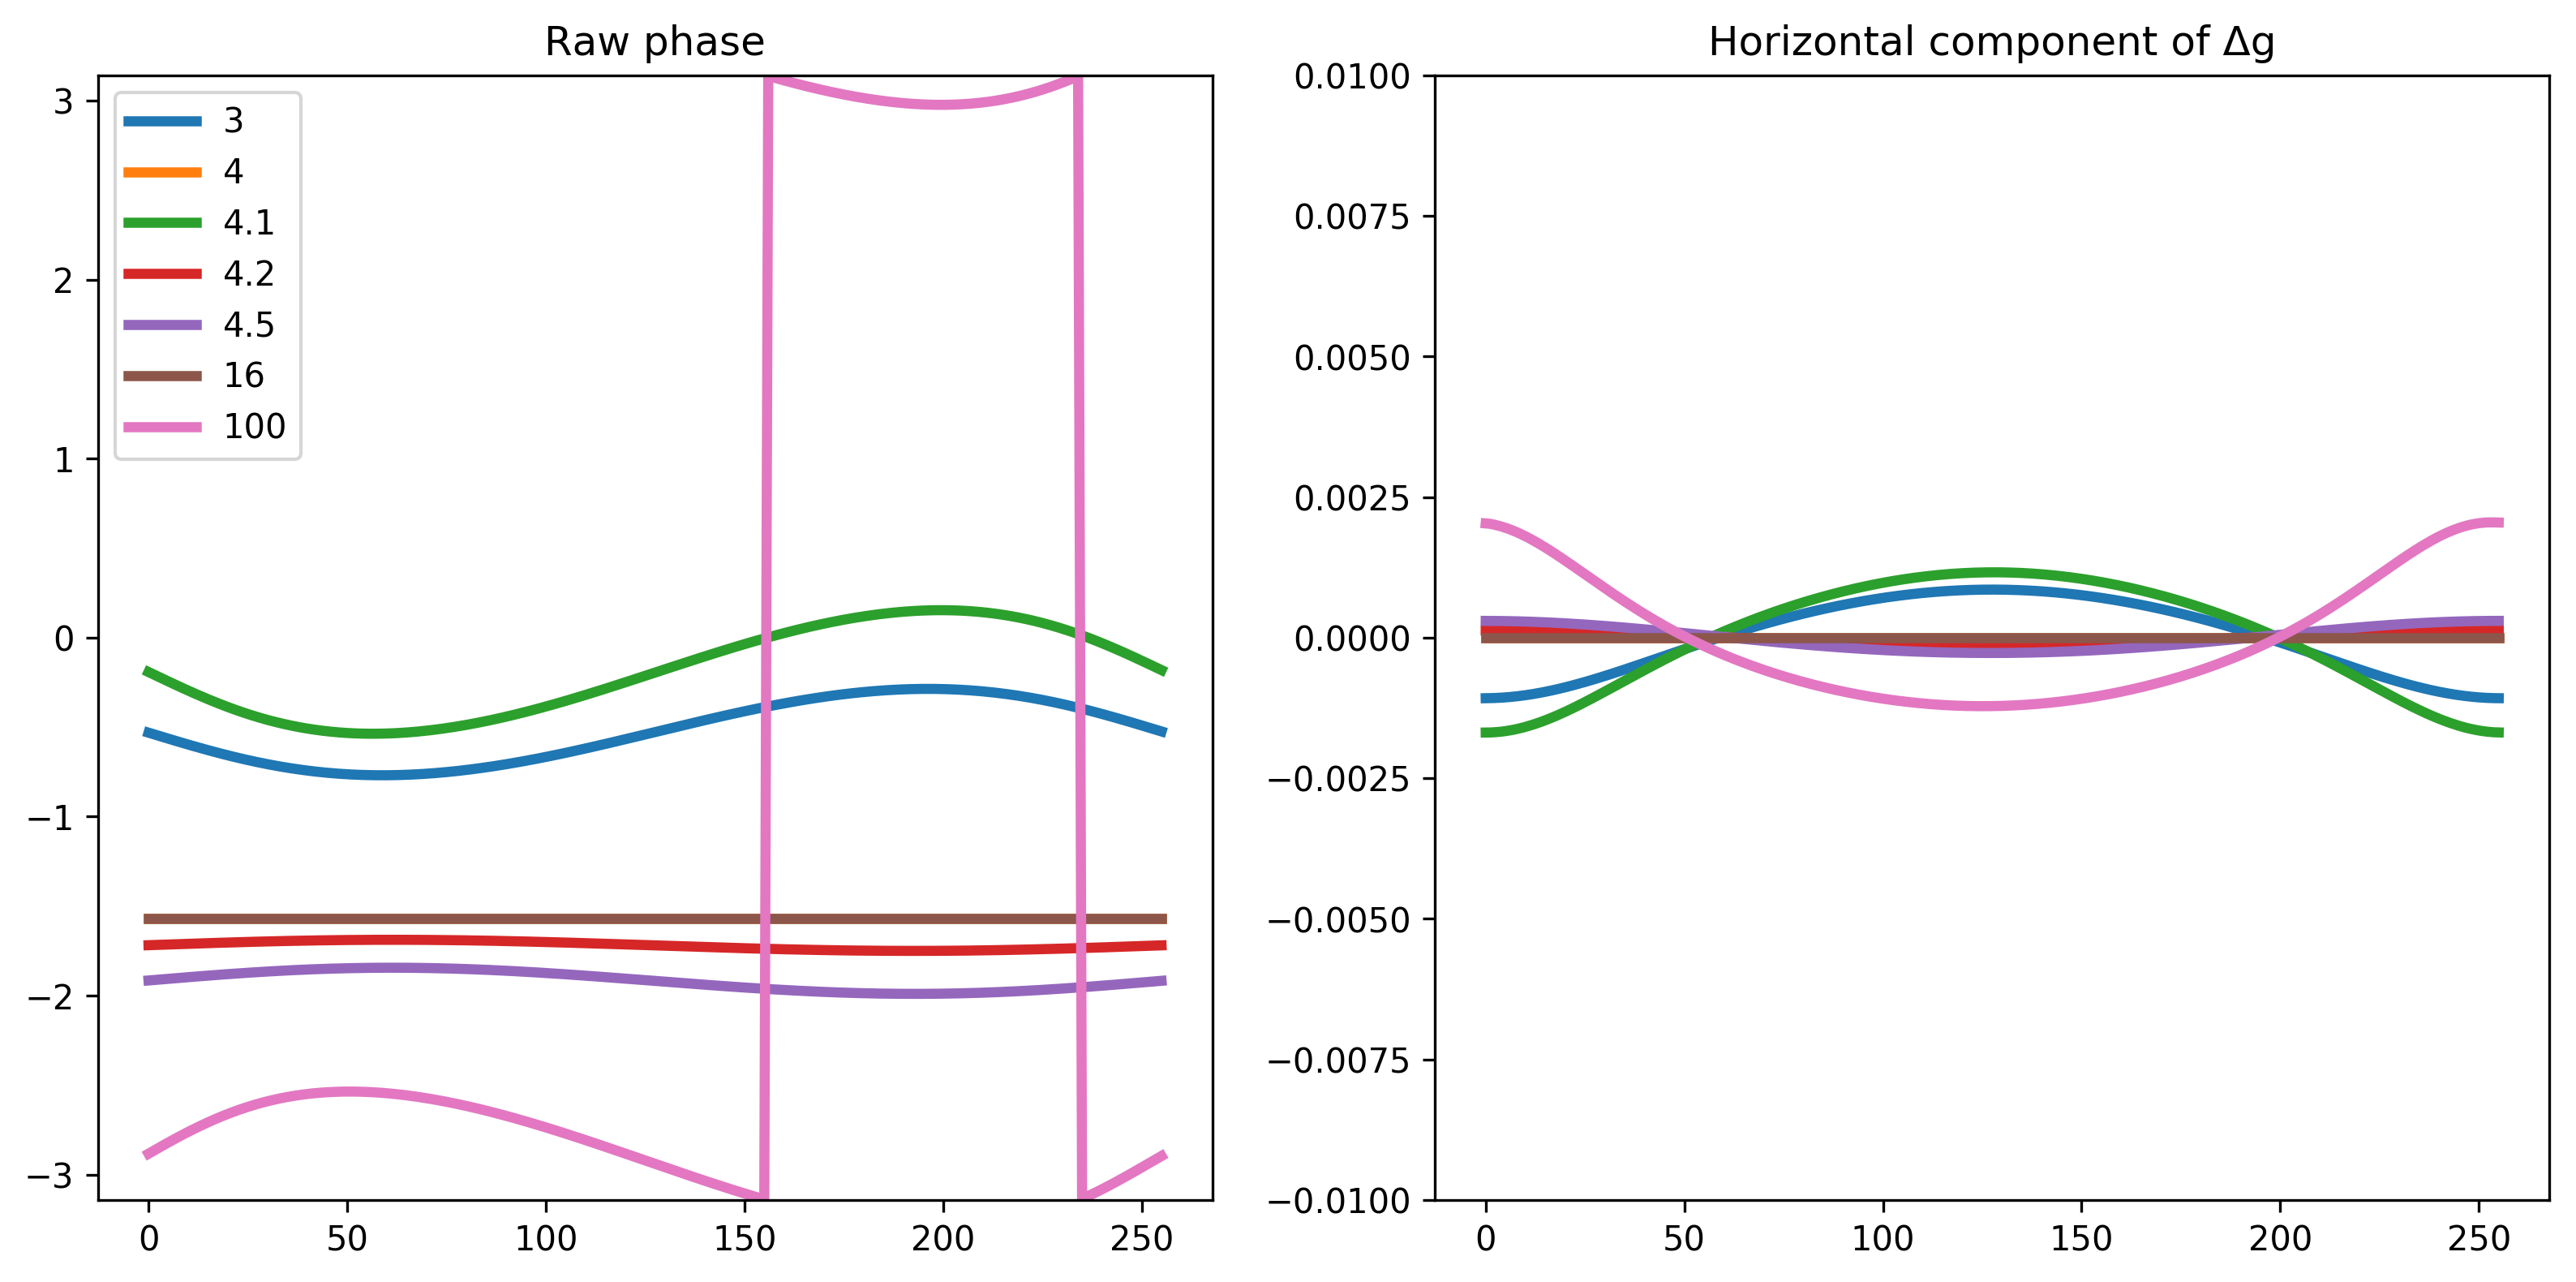
\includegraphics[scale=0.5]{Figures/Test_2_test_results.png}
\caption{}
\label{fig:Test_2_Test_results}
\end{center}
\end{figure}

\textbf{\cref{T:T_Phase-Extraction-Known-Strain}} from TestPlan document

\begin{figure}[H]
\begin{center}
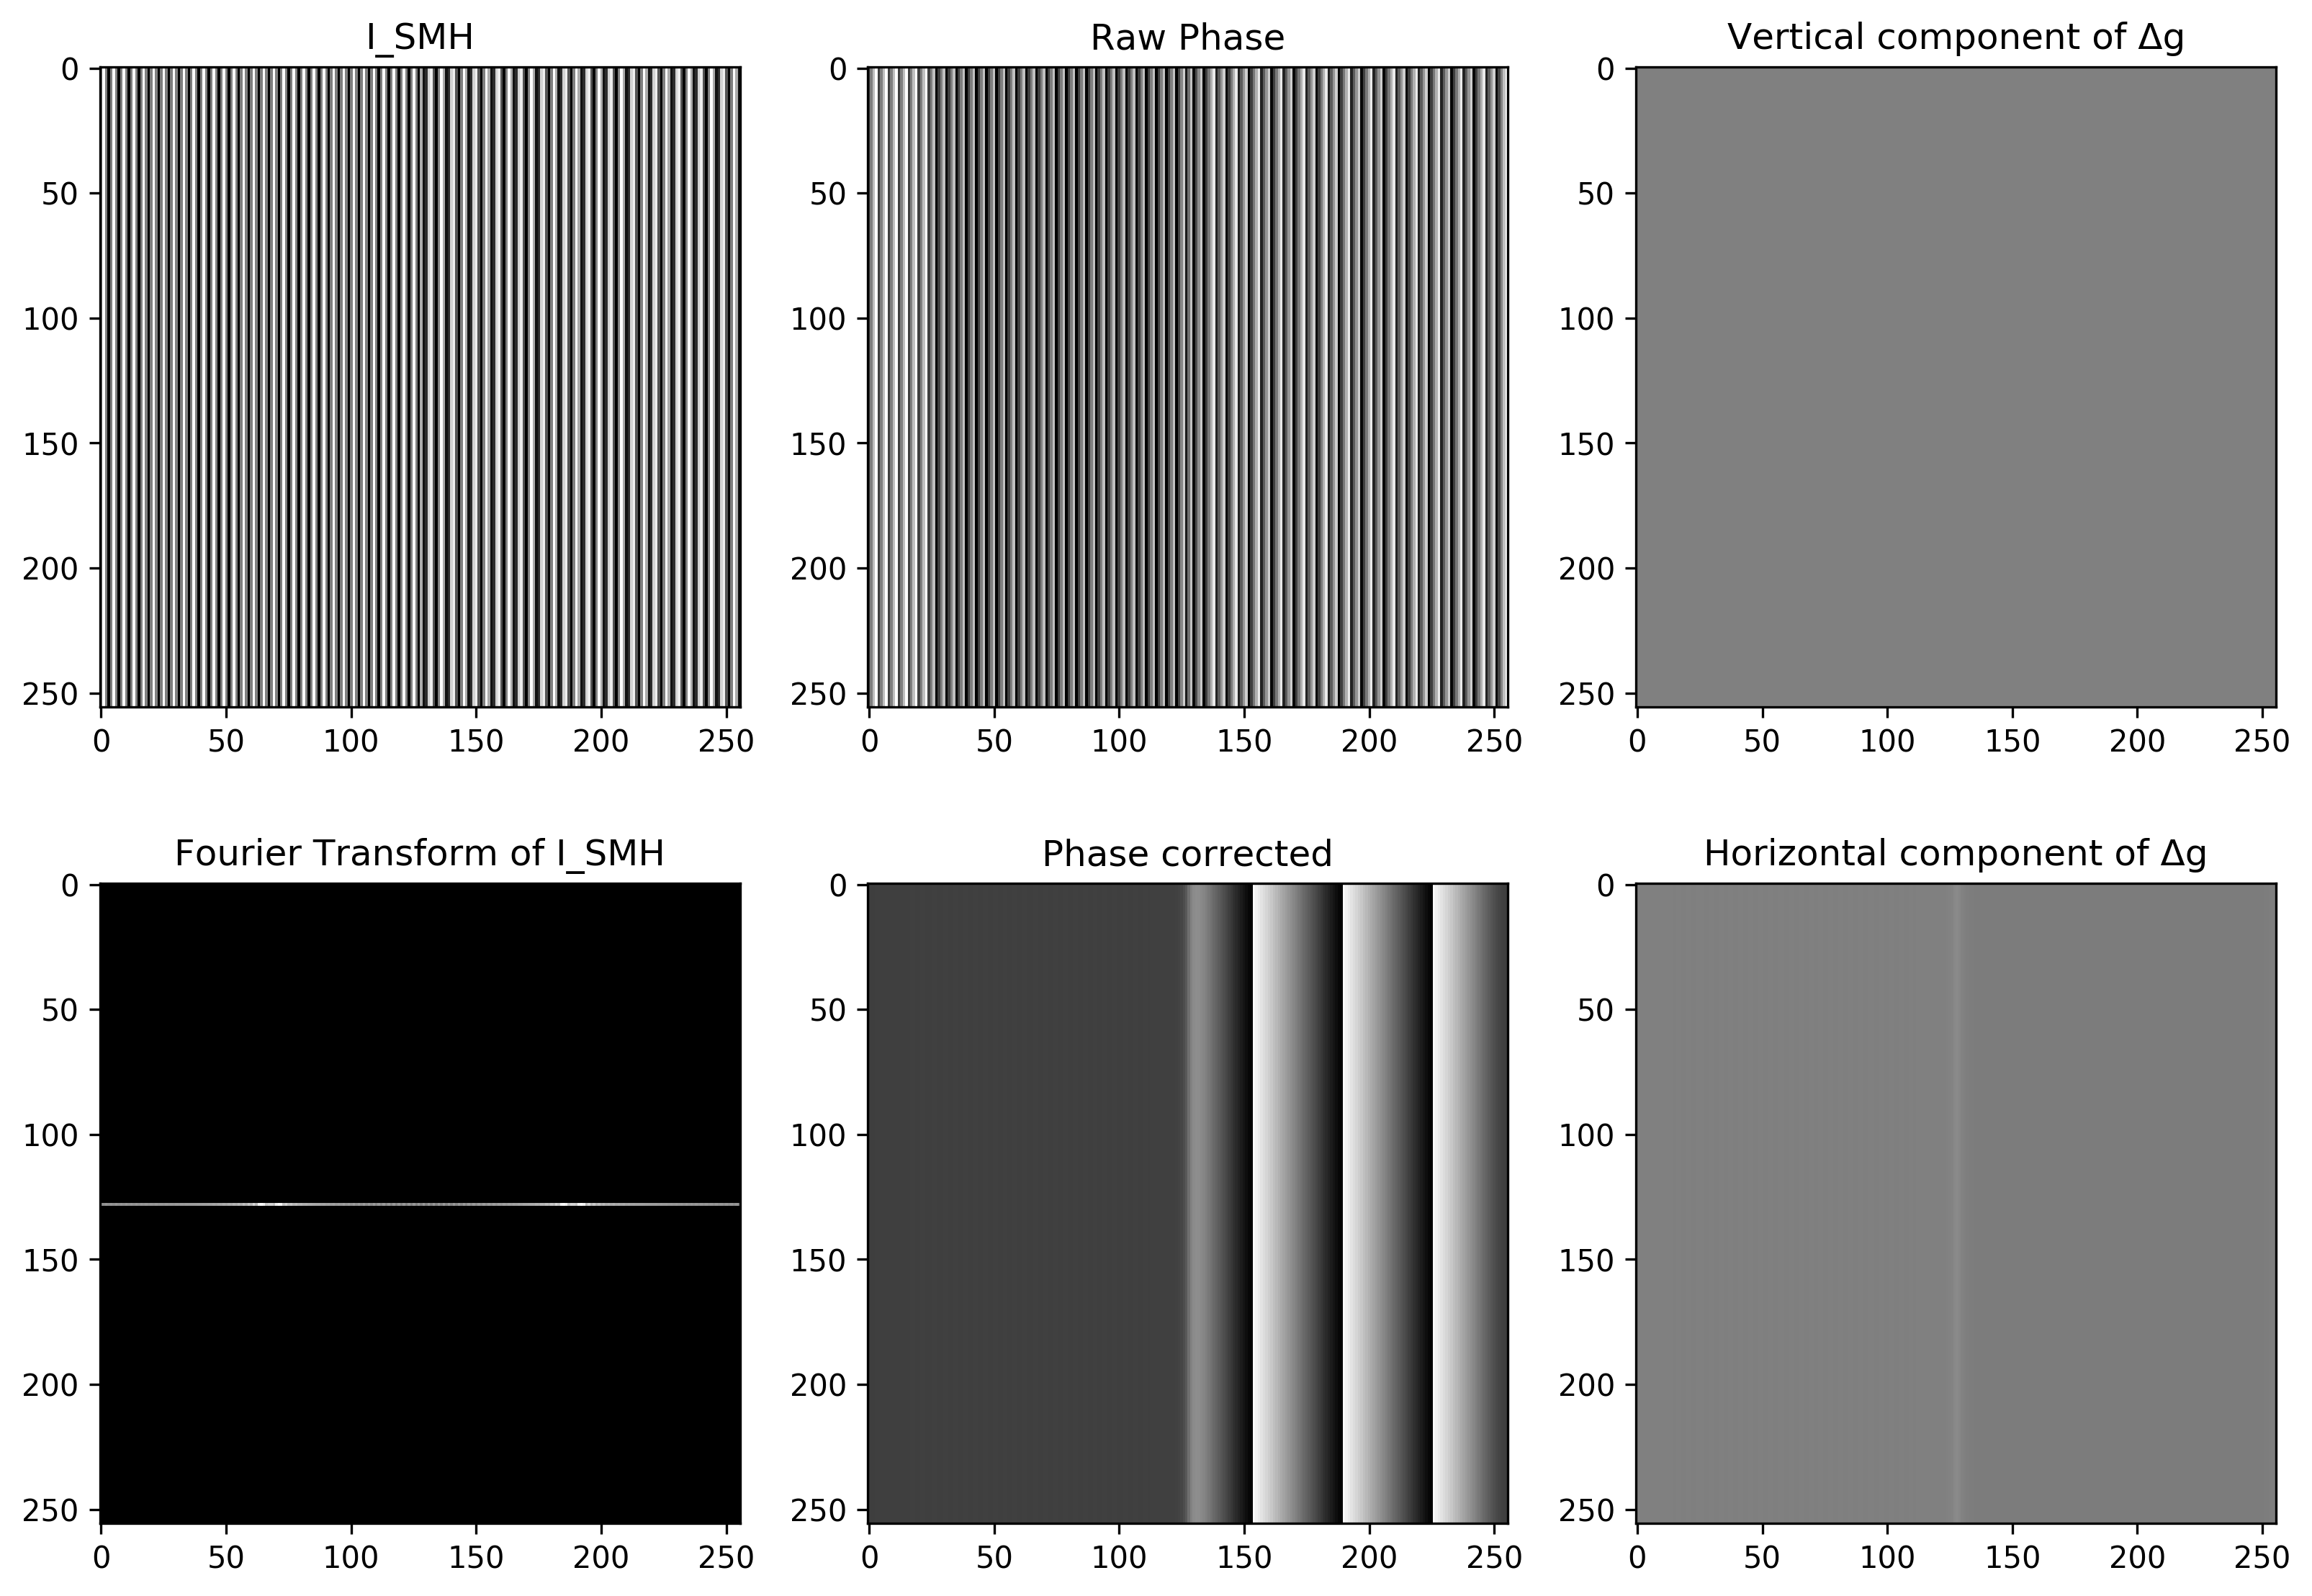
\includegraphics[scale=0.5]{Figures/Test_3_explanation.png}
\caption{}
\label{fig:Test_3_explaination}
\end{center}
\end{figure}

\begin{figure}[H]
\begin{center}
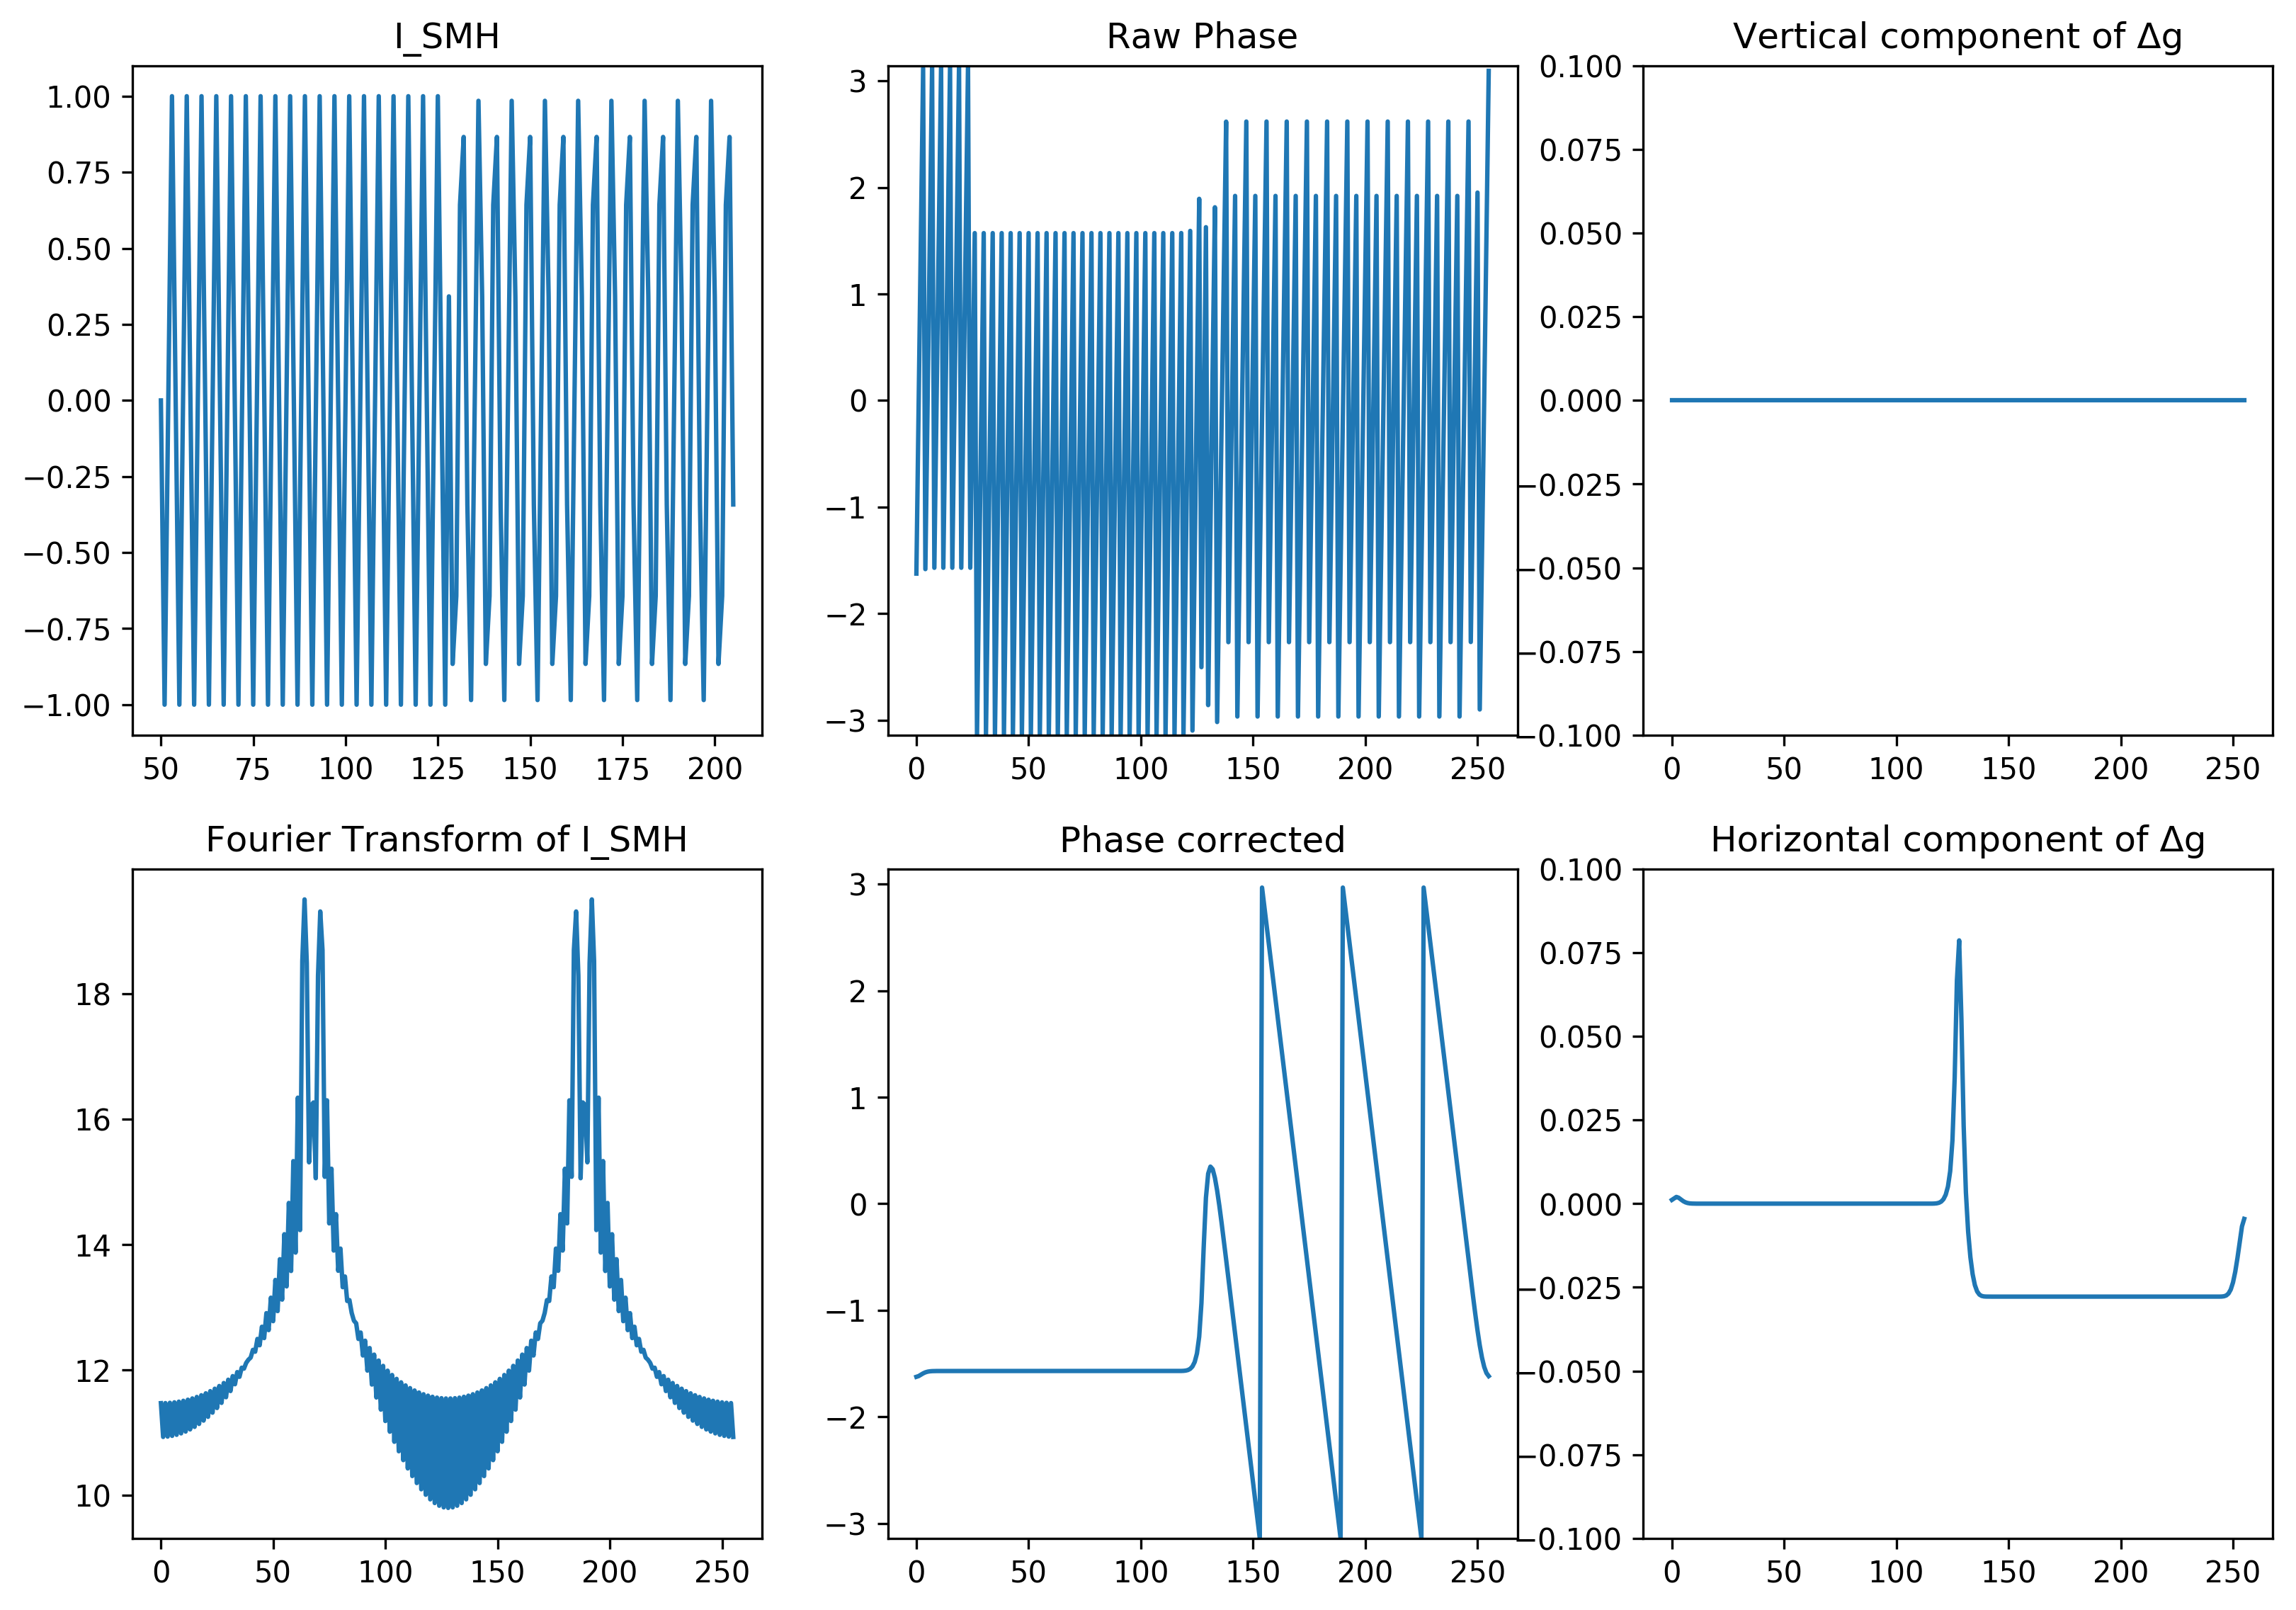
\includegraphics[scale=0.5]{Figures/Test_3_explanation_1D.png}
\caption{}
\label{fig:Test_3_explaination_1D}
\end{center}
\end{figure}

\begin{figure}[H]
\begin{center}
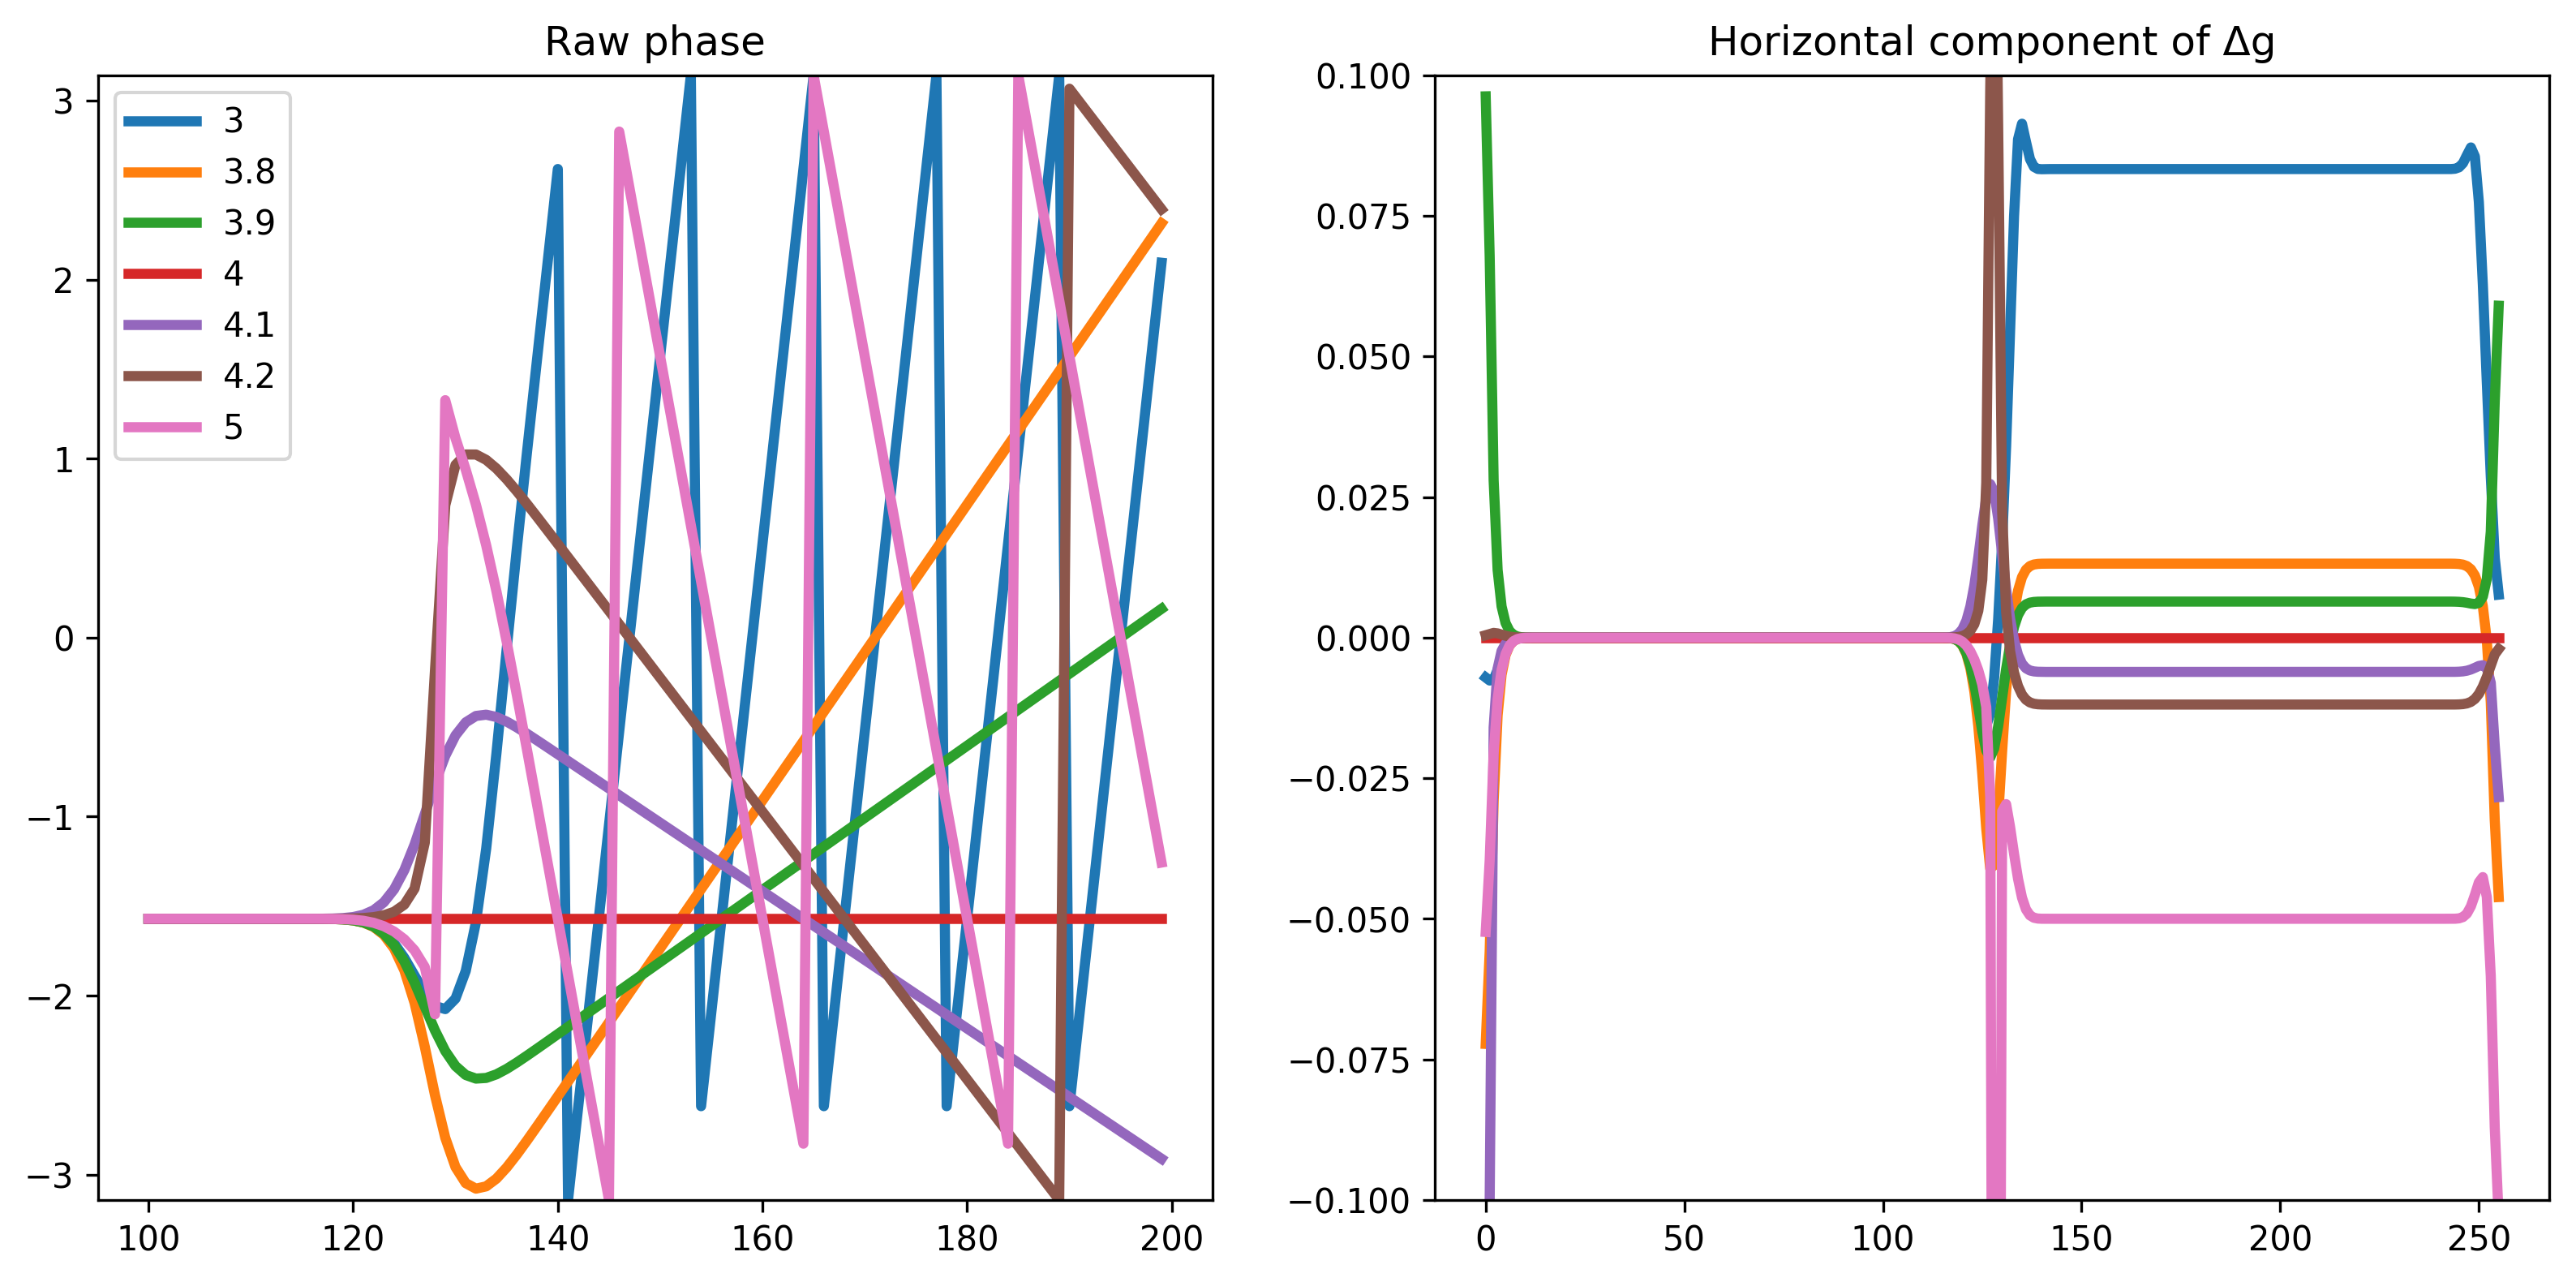
\includegraphics[scale=0.5]{Figures/Test_3_test_results.png}
\caption{}
\label{fig:Test_3_test_results}
\end{center}
\end{figure}

\section{Nonfunctional Requirements Evaluation}

Nonfunctional Requirements have not been addressed for the moment.
	
\section{Comparison to Existing Implementation}	

No other equivalent open-access software has been identified for a comparison. sMoir{\'e} program (available on \href{https://www.hremresearch.com/}{HREM website}) is a good candidate but a licence must be bought in order to use the software. The licence purchase is not an option, moreover all aspects of \progname{} are not covered by sMoir{\'e}.

The GPA algorithm used in \progname{} could be however compared to other open-access GPA software and is planned to be performed. Nevertheless, most of them are plug-ins for Digital Micrograph software therefore an interface must be designed to perform a comparison with \progname{}. 

\section{Unit Testing}



\section{Changes Due to Testing}

Mask function 

\section{Automated Testing}
		
\section{Trace to Requirements}
		
\section{Trace to Modules}		

\section{Code Coverage Metrics}

\bibliographystyle{ieee}

\bibliography{TestReport}

\end{document}